\documentclass[../5RO17_TP1.tex]{subfiles}

\begin{document}
\subsection{Question 2}
\noindent Étant donné qu'une \textbf{homographie} contient 8 degrés de liberté, représentés par 8 inconnues, au moins 4 points $\mathbf{p}_{i} = \begin{pmatrix} x & y \end{pmatrix}$ avec des coordonnées $x$ et $y$ sont nécessaires. Plus de points peuvent être utilisés, mais dans ce cas, la solution ne sera pas unique.\\

\noindent Le choix des points est nécessaire et essentiel pour l'application de l'homographie. Normalement, ces points sont définis à l'aide d'algorithmes. Dans ce travail pratique, cependant, les points seront choisis manuellement et sont notés ci-dessus :
\begin{table}[H]
    \centering
    \caption{Points Homographie}
    \label{tab_homography_points}
    \begin{subtable}[t]{0.475\textwidth}
        \centering
        \begin{tabular}{ccc}
            - & $x$ & $y$\\
            \hline
            $\mathbf{p}_{s_{1}} = \begin{pmatrix} x_{s_{1}} & y_{s_{1}} \end{pmatrix}$ & 120 & 023\\
            $\mathbf{p}_{s_{2}} = \begin{pmatrix} x_{s_{2}} & y_{s_{2}} \end{pmatrix}$ & 073 & 287\\
            $\mathbf{p}_{s_{3}} = \begin{pmatrix} x_{s_{3}} & y_{s_{3}} \end{pmatrix}$ & 409 & 299\\
            $\mathbf{p}_{s_{4}} = \begin{pmatrix} x_{s_{4}} & y_{s_{4}} \end{pmatrix}$ & 386 & 022\\
            \hline
        \end{tabular}
        \caption{Points Source}
    \end{subtable}
    \hfill
    \begin{subtable}[t]{0.475\textwidth}
        \centering
        \begin{tabular}{ccc}
            - & $x$ & $y$\\
            \hline
            $\mathbf{p}_{d_{1}} = \begin{pmatrix} x_{d_{1}} & y_{d_{1}} \end{pmatrix}$ & 083 & 000\\
            $\mathbf{p}_{d_{2}} = \begin{pmatrix} x_{d_{2}} & y_{d_{2}} \end{pmatrix}$ & 083 & 333\\
            $\mathbf{p}_{d_{3}} = \begin{pmatrix} x_{d_{3}} & y_{d_{3}} \end{pmatrix}$ & 416 & 333\\
            $\mathbf{p}_{d_{4}} = \begin{pmatrix} x_{d_{4}} & y_{d_{4}} \end{pmatrix}$ & 416 & 000\\
            \hline
        \end{tabular}
        \caption{Points Destination}
    \end{subtable}
\end{table}
\begin{remark}
    Toutes les coordonnées sont données en pixels.
\end{remark}
\noindent Pour maximiser l'effet de recadrage, les points de destination ont été choisis de façon à ce que le carré ait pour dimension le minimum entre l'hauteur, 333 pixels,  et la largeur, 500 pixels, de l'image. Dans ce cas, cependant, le carré aura 333 pixels de largeur et sera centré sur le centre de l'image.\\

\noindent Ci-dessous, les points sont présentés sur l'image source et sur l'image destination:
\begin{figure}[ht]
    \centering
    \begin{subfigure}[b]{0.45\textwidth}
        \centering
        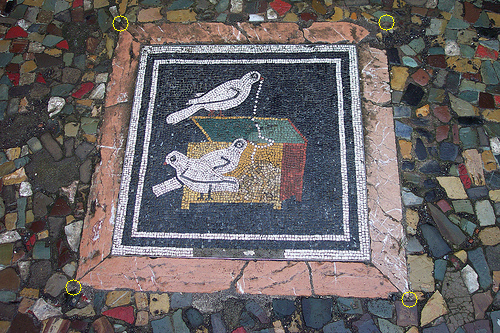
\includegraphics[width=\linewidth]{images/image_source_points.png}
        \caption{Image Source}
    \end{subfigure}\hfill
    \begin{subfigure}[b]{0.45\textwidth}
        \centering
        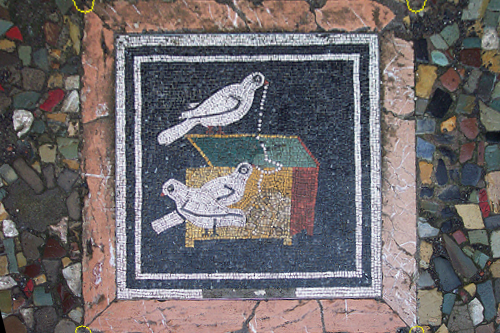
\includegraphics[width=\linewidth]{images/image_corrected.png}
        \caption{Image Destination}
    \end{subfigure}
    \caption{Points choisit pour l'Homographie}
    \label{fig:sidebyside}
\end{figure}

\noindent Dans cette approche, il faut au moins 4 correspondances de points entre l'image source $\mathbf{p}_{s_{i}}$ et l'image destination $\mathbf{p}_{d_{i}}$ afin d'établir un système d'équations à résoudre par une méthode telle que la Transformation Linéaire Directe.\\

\noindent Les points choisis sont les points d'intérêt de la transformation requise, les quatres coins du carré à transformer. Ils ont été choisis avec l'aide de l'interface graphique dejà dsponible, puis maintenus pour garantir la reproductibilité des résultats.
\end{document}
